\documentclass[12pt,a4paper]{scrartcl} 
\usepackage[utf8]{inputenc}
\usepackage[english,russian]{babel}
\usepackage{indentfirst}
\usepackage{misccorr}
\usepackage{graphicx}
\usepackage{indentfirst}
\usepackage{amsmath}
\begin{document}
 \begin{titlepage}
  \begin{center}
   \large
   МИНИСТЕРСТВО НАУКИ И ВЫСШЕГО ОБРАЗОВАНИЯ РОССИЙСКОЙ ФЕДЕРАЦИИ
   
   Федеральное государственное бюджетное образовательное учреждение высшего образования
   
   \textbf{АДЫГЕЙСКИЙ ГОСУДАРСТВЕННЫЙ УНИВЕРСИТЕТ}
   \vspace{0.25cm}
   
   Инженерно-физический факультет
   
   Кафедра автоматизированных систем обработки информации и управления
   \vfill

   \vfill
   
   \textsc{Отчет по практике}\\[5mm]
   
   {\LARGE Программаная реализация численного метода \textit{Интерполировать функцию, используя многочлен Лагранжа (количество точек задается из программы)}}
   \bigskip
   
   1 курс, группа 1ИВТ1-2
  \end{center}
  \vfill
  
  \newlength{\ML}
  \settowidth{\ML}{«\underline{\hspace{0.7cm}}» \underline{\hspace{2cm}}}
  \hfill\begin{minipage}{0.5\textwidth}
   Выполнила:\\
   \underline{\hspace{\ML}} Т.\,И.~Андрощук\\
   «\underline{\hspace{0.7cm}}» \underline{\hspace{2cm}} 2023 г.
  \end{minipage}%
  \bigskip
  
  \hfill\begin{minipage}{0.5\textwidth}
   Руководитель:\\
   \underline{\hspace{\ML}} С.\,В.~Теплоухов\\
   «\underline{\hspace{0.7cm}}» \underline{\hspace{2cm}} 2023 г.
  \end{minipage}%
  \vfill
  
  \begin{center}
   Майкоп, 2023 г.
  \end{center}
 \end{titlepage}
 

\section{Введение}
\label{sec:intro}


\subsection{Формулировка цели}
Целью данной работы является написание программы для интерполирования функции, используя многочлен Лагранда.

\subsubsection{Теория}
Интерполяционный многочлен Лагранжа — многочлен минимальной степени, принимающий данные значения в данном наборе точек. Для n+1 пар чисел (x0, y0), (x1, y1),…, (xn, yn), где все xj различны, существует единственный многочлен L(x) степени не более n, для которого L(xj) = yj. В простейшем случае (n=1) — это линейный многочлен, график которого — прямая, проходящая через две заданные точки.
Li(x) обладают следующими свойствами:
\begin{enumerate}
 \item являются многочленами степени n;
 \item Li(xi) = 1;
 \item Li(xj) = 0 при j ≠ i.
\end{enumerate}


\section{Ход работы}
\label{sec:exp}

\subsection{Код приложения}
\label{sec:exp:code}
\begin{verbatim}
#include <iostream>
using namespace std;

struct Data { double x, y; };

double interpolate(Data f[], int n, double xi) {
    double result = 0;
    for (int i = 0; i < n; i++) {
        double term = f[i].y;
        for (int j = 0; j < n; j++) {
            if (j != i) term *= (xi - f[j].x) / (f[i].x - f[j].x);
        }
        result += term;
    }
    return result;
}

int main() {
    const int n = 4;

    Data f[n] = {
     { 0, 2 },
     { 1, 3 },
     { 2, 12 },
     { 5, 147 }
    };

    double x1 = 0,
        x2 = 5,
        dx = 0.125;
    cout.width(20); cout << "X"; cout.width(20); cout << "Y" << endl;
    for (double x = x1; x <= x2; x += dx) {
        double y = interpolate(f, n, x);
        cout.width(20); cout.precision(14); cout << x;
        cout.width(20); cout.precision(14); cout << y << endl;
    }

    cin.get();
    return 0;
}
\end{verbatim}

\subsection{Формулы}
\label{sec:mathexample}

Формула Лангранжа: \(L(x)=\sum\limits_{i=0}^n y_{i}l_{i}(x)\):
\begin{equation}\label{eq:solv}
 l_{i}(x)=\frac{x-x_{0}}{x_{i}-x_{0}} ... \frac{x-x_{i-1}}{x_{i}-x_{i-1}}*\frac{x-x_{i+1}}{x_{i}-x_{i+1}} ... \frac{x-x_{n}}{x_{i}-x_{n}}.
\end{equation}



\section{Скриншоты программы}

\label{sec:picexample}
\begin{figure}[h]
	\begin{center}
    \begin{minipage}{0.39\linewidth}
	  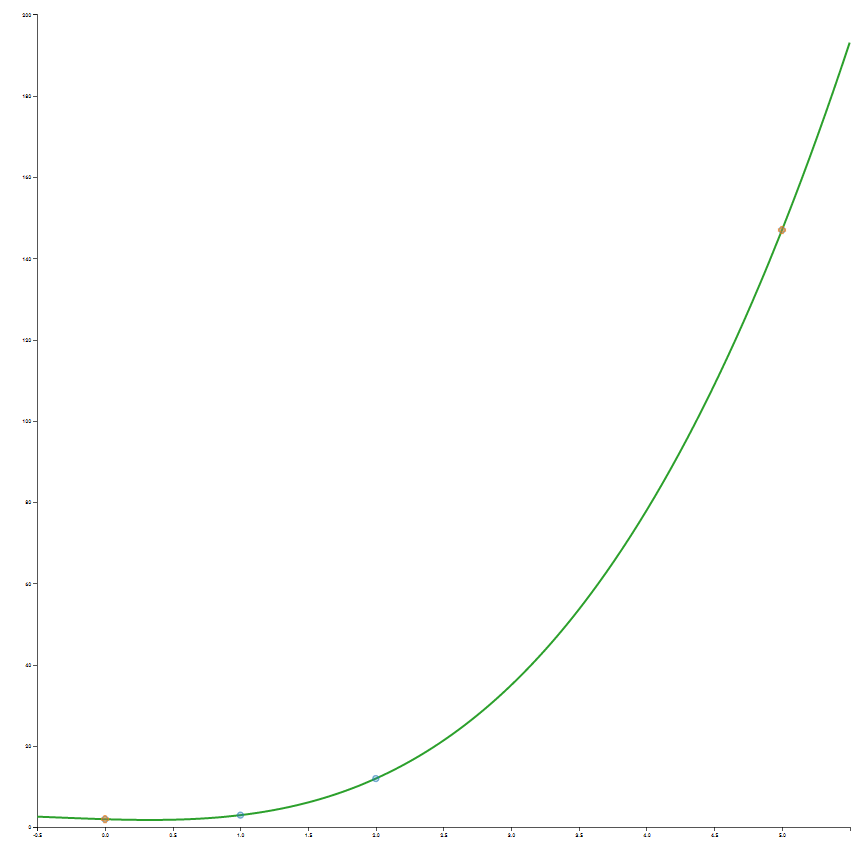
\includegraphics[width=0.6\textwidth]{График.PNG}
	  \caption{График}\label{fig:par}
    \end{minipage}
    \hfill
    \begin{minipage}{0.39\linewidth}
	  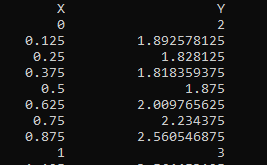
\includegraphics[width=1\textwidth]{Решение.PNG}
	  \caption{Решение}\label{fig:par}
    \end{minipage}
    \end{center}
\end{figure}



\begin{thebibliography}{9}
\bibitem{Knuth-2003}Кнут Д.Э. Всё про \TeX. \newblock --- Москва: Изд. Вильямс, 2003 г. 550~с.
\bibitem{Lvovsky-2003}Львовский С.М. Набор и верстка в системе \LaTeX{}. \newblock --- 3-е издание, исправленное и дополненное, 2003 г.
\bibitem{Voroncov-2005}Воронцов К.В. \LaTeX{} в примерах. 2005 г.
\end{thebibliography}

\end{document}
